We now dissect the production estimator of Section~\ref{sec:framework} and locate three distinct normalization defects. All three violate the same requirement---every probability measure entering the per-event likelihood must be counted identically wherever the corresponding axis is integrated, in the numerator as in the selection normalization---but they act through different channels, span five orders of magnitude in size, and pull the posterior in opposite directions. This section states each defect and its predicted signature; Section~\ref{sec:pitfall:chain} assembles them into a single falsifiable prediction, which Sections~\ref{sec:coverage} and \ref{sec:realdata} test.

\subsection{Prior inconsistency in the host-redshift kernel}
\label{sec:pitfall:kernel}

The in-catalogue numerator marginalizes each candidate host's unknown true redshift $z$ against the bare photometric likelihood $\mathcal{N}(z;z_g,\sigma_z^2)$, where $z_g$ is the catalogue redshift: it treats every true redshift within the measurement scatter as equally probable a priori. Everywhere else the estimator asserts the opposite. The selection normalization $D(h)$, its out-of-catalogue part $\beta_{\bar{G}}(h)$, and the completion numerator $B_{\mathrm{num}}(h)$ (Section~\ref{sec:framework}) all integrate over redshift against the detector-frame population measure
\begin{equation}
  w_{\mathrm{pop}}(z) \equiv \frac{1}{1+z}\,\frac{\mathrm{d}V_{\mathrm{c}}}{\mathrm{d}z},
  \label{eq:pitfall:wpop}
\end{equation}
the uniform-in-comoving-volume host prior with cosmological time dilation \citep{Gray:2019ksv,Mandel:2018mve}. The numerator is therefore prior-inconsistent with its own denominator: the population prior is counted once on one side of the likelihood ratio and zero times on the other.

The consequence is the classical Eddington--Malmquist bias transcribed to redshift space \citep{Eddington1913,Malmquist1922}.
Because the measure~\eqref{eq:pitfall:wpop} rises steeply with $z$---there is more volume, hence there are more potential hosts, behind an observed redshift than in front of it---a galaxy observed at $z_g$ is more probably a higher-redshift galaxy scattered down than a lower-redshift galaxy scattered up. Omitting the prior under-estimates every host redshift, at leading order by
\begin{equation}
  \delta z_{\mathrm{Edd}} = \sigma_z^{2}\, s(z_g),
  \qquad
  s(z) \equiv \frac{\mathrm{d}\ln w_{\mathrm{pop}}}{\mathrm{d}z},
  \label{eq:pitfall:eddz}
\end{equation}
% src: docs/derivations/G2b_host_z_volume_prior.md Eq. (2.1)
and, propagated through the distance--redshift relation, it biases the Hubble constant low by
\begin{equation}
  \Delta h \simeq -\,h \left.\frac{\mathrm{d}\ln d_L}{\mathrm{d}z}\right|_{\bar{z}} \sigma_z^{2}\, s(\bar{z})
  \;\equiv\; -\,C(\bar{z})\,\sigma_z^{2},
  \label{eq:pitfall:hbias}
\end{equation}
% src: docs/derivations/G2b_host_z_volume_prior.md Eq. (2.3); d ln d_L/dz = d ln[(1+z)I(z)]/dz is h-independent
where $\bar{z}$ is a representative detected-host redshift; the derivation, the population-averaging of $C(\bar z)$, and the exact-quadrature cure are given in Appendix~\ref{sec:app:voldeconv}.

Equation~\eqref{eq:pitfall:hbias} is quantitatively verified. In single-host synthetic tests (flat $\Lambda$CDM, $\Omega_{\mathrm{m}}=0.3$, true $h=0.72$, complete catalogue) the measured maximum-a-posteriori biases are % src: docs/derivations/G2b_host_z_volume_prior.md preamble + section 2.3
$\Delta h = -0.0016$, $-0.0064$, $-0.023$ and $-0.046$ at $\sigma_z = 0.005$, $0.015$, $0.035$ and $0.050$; % src: docs/derivations/G2b_host_z_volume_prior.md section 2.3
after subtracting a $\sigma_z$-independent estimator floor of $\approx -0.002$ they scale as $1:4.8:10.0$ against $\sigma_z^2 = 1:5.44:11.1$, i.e.\ the quadratic law holds to $\sim$10~per~cent, % src: docs/derivations/G2b_host_z_volume_prior.md section 2.3
and the implied coefficient $-\Delta h/\sigma_z^2 \approx 17$--$20$ matches $C(\bar z)$ at $\bar z \approx 0.25$--$0.27$, inside the synthetic detected population. % src: docs/derivations/G2b_host_z_volume_prior.md section 2.3
The same offset, rigid across realizations, collapses empirical P--P coverage to $\approx 0$--3~per~cent at every injected truth (Section~\ref{sec:coverage}). % src: .planning/INDEPENDENT-VERIFICATION-REPORT-20260701.md section 7.1

For a GLADE-like catalogue the effect is not even perturbative. At a host redshift $z_g = 0.05$ the expansion parameter of Eq.~\eqref{eq:pitfall:eddz} is $\sigma_z\, s(z_g) = 1.33$ already at $\sigma_z = 0.035$, % src: docs/derivations/G2b_host_z_volume_prior.md section 2.3
and the exact posterior-mean redshift shift, while saturating below the quadratic law ($+0.0325$ exact versus $+0.0467$ at leading order for $\sigma_z=0.035$), remains $\gtrsim 60$~per~cent of $z_g$ itself. % src: docs/derivations/G2b_host_z_volume_prior.md section 2.3 table
A kernel that mis-locates every host by over half its redshift does not average out over events; it coherently distorts the entire in-catalogue channel.

\subsection{The completion term's missing sky marginal}
\label{sec:pitfall:sky}

The completion term requires the GW measurement likelihood marginalized over the isotropic sky prior $p(\Omega) = 1/(4\pi)$ of the out-of-catalogue host population \citep{Gray:2019ksv}. The production code instead evaluated the three-dimensional Gaussian approximation to the GW likelihood---in the coordinates $(\phi,\theta,u)$, with $u = d_L/\hat{d}_L$ the luminosity-distance fraction and covariance $\Sigma$ from the per-event Fisher matrix---at its sky maximum, substituting the \emph{peak coordinate density} for the sky \emph{marginal}. For the narrow localizations at hand the exact isotropic marginal factorizes (Appendix~\ref{sec:app:sky}) as
\begin{equation}
  \bar{p}_{\mathrm{GW}}(u)
  = \frac{\sin\hat{\theta}}{4\pi}\,
  \mathcal{N}\!\left(u;\,1,\,\Sigma_{uu}\right),
  \label{eq:pitfall:skymarg}
\end{equation}
% src: docs/derivations/G2a_completion_sky_marginal_4pi.md Eq. (10)
with $\hat{\theta}$ the estimated polar angle and $\Sigma_{uu} = \sigma_{d_L}^2/\hat{d}_L^{\,2}$ the \emph{marginal} fractional-distance variance. The peak evaluation replaces the prefactor of Eq.~\eqref{eq:pitfall:skymarg} by $\approx (2\pi\sigma_\phi\sigma_\theta)^{-1}$, where $\sigma_\phi,\sigma_\theta$ are the sky-localization widths---an over-weighting of $B_{\mathrm{num}}$ by $2/(\sigma_\phi\sigma_\theta) \approx 1.6\times10^{3}$ at a $2\degr$ sky error % src: docs/derivations/G2a_completion_sky_marginal_4pi.md section 7 item 5
and $\approx 1.8\times10^{5}$ at the median EMRI localization of $0.2\,\mathrm{deg}^2$ in our simulated campaign. % src: docs/derivations/G2a_completion_sky_marginal_4pi.md sections 4 and 7
Crucially, this factor multiplies $B_{\mathrm{num}}$ alone, not the in-catalogue term $\beta_G L_{\mathrm{cat}}$, so it does not cancel in the per-event mixture $p_i(h) = [\beta_G(h) L_{\mathrm{cat}}(h) + B_{\mathrm{num}}(h)]/D(h)$: it silently converts the estimator into a completion-dominated one, with the catalogue information suppressed by three to five orders of magnitude.

A subtlety survives the $1/(4\pi)$ repair. The Fisher Gaussian is a density with respect to the coordinate measure $\mathrm{d}\phi\,\mathrm{d}\theta$, not the solid-angle measure $\mathrm{d}\Omega = \sin\theta\,\mathrm{d}\theta\,\mathrm{d}\phi$, so the exact marginal retains the Jacobian $\sin\hat{\theta}$ of Eq.~\eqref{eq:pitfall:skymarg}; implementing the marginal as $1/(4\pi)$ alone over-weights the completion channel by $1/\sin\hat{\theta}$ per event (median $\approx 1.15$, mean $\pi/2$ for isotropic events). % src: docs/derivations/G2a_completion_sky_marginal_4pi.md sections 4--5
This residual is $h$-independent per event but, like the parent defect, re-weights the catalogue--completion mixture; it is three orders of magnitude below the peak-density error and is quantified, with the full error budget of the factorization, in Appendix~\ref{sec:app:sky}.

\subsection{The global selection sum: a residual $h$-tilt}
\label{sec:pitfall:global}

The third defect afflicts the ``global'' normalization mode, in which the in-catalogue likelihood divides a local, event-adjacent sum by a discrete detection-weighted sum over the whole catalogue,
\begin{equation}
  \Sigma_{\mathrm{global}}(h) = \sum_{g} w_g\, p_{\mathrm{det}}\big(d_L(z_g,h)\big),
  \label{eq:pitfall:sigmaglobal}
\end{equation}
% src: .planning/gate/G1_beta_g_check.md (definition of the discrete GLADE sum)
with $w_g$ the per-galaxy rate weights of Section~\ref{sec:framework}. Its validity rests on treating the catalogue as a Monte Carlo draw of the completeness-weighted galaxy density, so that $\Sigma_{\mathrm{global}}(h) \approx C\,\beta_G(h)$ with $C$ independent of $h$ and cancelling in the posterior. We tested this cancellation directly on GLADE+ \citep{Dalya:2021ewn} by evaluating both sides over 14 values of $h \in [0.60, 0.86]$ (Fig.~\ref{fig:betag}; Appendix~\ref{sec:app:betag}). % src: .planning/gate/G1_beta_g_check.md
The raw ratio $\Sigma_{\mathrm{global}}/\beta_G$ grows by a factor 2.48 across the grid. % src: .planning/gate/G1_beta_g_check.json (raw ratio 8.9567 -> 22.1973)
Most of this is benign: a fixed galaxy set implies a comoving number density $n_{\mathrm{gal}}(h) \propto 1/V_{\mathrm{c}} \propto h^3$, and $(0.86/0.60)^3 = 2.94$ cancels between the discrete numerator and denominator of $L_{\mathrm{cat}}$. % src: .planning/gate/G1_beta_g_check.md finding 1
After dividing out $h^3$, however, a smooth, monotonic residual tilt of $-17.2$~per~cent end-to-end remains ($+8.7$~per~cent at $h=0.60$ to $-8.7$~per~cent at $h=0.86$, normalized at $h=0.72$): % src: .planning/gate/G1_beta_g_check.json (end_to_end_tilt_h3_corrected = -0.1719; shape 1.0854 -> 0.9135)
a real $h$-dependent mismatch between the discrete completeness-weighted catalogue content and the continuous completeness-model integral; its candidate origins (completeness modelling, large-scale structure against the constant-comoving-density assumption, the mass-integrated rate surrogate) are discussed in Appendix~\ref{sec:app:betag}. % src: .planning/gate/G1_beta_g_check.md finding 2

Unlike a per-event noise term, this tilt multiplies the in-catalogue channel of \emph{every} event coherently: after $N \approx 500$ events the accumulated distortion of the log-likelihood is enormous. % src: .planning/gate/G1_beta_g_check.md finding 3
Estimators that normalize locally---dividing the event-adjacent numerator sum by the event-adjacent selection sum over the same galaxies (Section~\ref{sec:estimators})---never form $\Sigma_{\mathrm{global}}$ and are structurally immune.

\begin{figure}
  \centering
  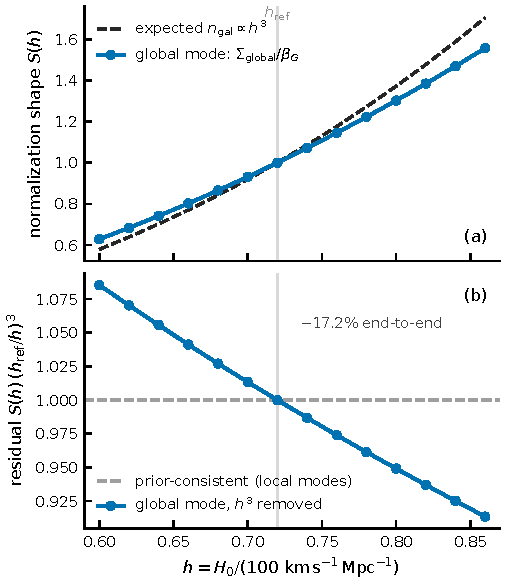
\includegraphics[width=\columnwidth]{figures/fig_beta_g.pdf}
  \caption{Direct test of the global-mode cancellation
  $\Sigma_{\mathrm{global}}(h) \approx C\,\beta_G(h)$, Eq.~\eqref{eq:pitfall:sigmaglobal}, on GLADE+
  (14 values of $h \in [0.60,0.86]$, normalized at $h=0.72$). % src: .planning/gate/G1_beta_g_check.md
  The raw ratio grows by a factor 2.48 across the grid, dominated by the
  expected catalogue-density scaling $n_{\mathrm{gal}} \propto h^3$, which
  cancels in the likelihood ratio; after removing $h^3$ a smooth
  $-17.2$~per~cent end-to-end residual tilt remains, which does not cancel
  and coherently tilts the ``global''-mode in-catalogue channel once per
  event. % src: .planning/gate/G1_beta_g_check.json
  }
  \label{fig:betag}
\end{figure}

\subsection{Three defects, one prediction: the sign-flip chain}
\label{sec:pitfall:chain}

Ordered by magnitude, the three defects predict a distinctive progression under staged repair---distinctive because the two normalization errors have opposite signs, so fixing only the larger one must \emph{flip} the failure rather than remove it.

First, with the peak-density completion term inflated by $10^3$--$10^5$ (Section~\ref{sec:pitfall:sky}), the per-event likelihood is completion-dominated and the posterior on the real GLADE+ data rails at the upper edge of the search grid, $h = 0.86$, with essentially all posterior mass on the edge point. % src: results/commission_20260701/redteam/crux_results.json (MAP 0.86, edge_mass 1.0)
Second, restoring the isotropic $1/(4\pi)$ sky marginal \emph{alone} removes that inflation but leaves the in-catalogue channel prior-inconsistent: its numerator marginalizes the photometric scatter against the bare Gaussian while its global selection sum point-evaluates $p_{\mathrm{det}}$ at the catalogue redshifts and carries the $-17$~per~cent tilt of Section~\ref{sec:pitfall:global}. % src: docs/derivations/G2c_gray_a9_a10_mapping.md note C6; .planning/gate/G1_beta_g_check.md
The prediction is a railed posterior of the opposite sign---and on the identical data the $4\pi$-only configuration rails at the \emph{lower} grid edge, $h = 0.60$, again with all mass on the edge. % src: results/commission_20260701/redteam/derail_matrix_results.json (prod_global: MAP 0.60, edge_mass 0.99999990)
The completion fix is necessary but not sufficient. (Both rail modes are 100~per~cent edge-mass results at the endpoints of the grid, so the unconstrained modes may lie outside $[0.60,0.86]$.) % src: results/commission_20260701/redteam/derail_matrix_results.json
Third, restoring numerator--denominator prior consistency in the in-catalogue channel---by either of the two principled routes of Section~\ref{sec:estimators}, the local ratio-of-sums or the comoving-volume deconvolution of the host-redshift kernel---de-rails the posterior entirely: on the same 494-event subsample and seven-point grid, both peak at the injected $h = 0.73$ (posterior means $0.730$ and $0.740$, respectively). % src: results/commission_20260701/redteam/derail_matrix_results.json (local_ratio mean 0.7298; volume_deconv mean 0.7398); results/commission_20260701/redteam/crux_realdata.md (494 events, 7-point grid)
The two factors can also be separated: keeping the global denominator but making the kernel volume-consistent on both sides already de-rails to a peaked posterior at $h = 0.76$, and switching to the local denominator removes the remaining $+0.03$---the ablation is presented in Section~\ref{sec:postmortem}. % src: .planning/gate/G3_ablation_cube.json (volume_global MAP 0.76; local_ratio/volume_deconv MAP 0.73)

The sign flip is the diagnostic heart of this paper. A single mis-normalization would predict monotone improvement under repair; the observed up-rail~$\to$~down-rail~$\to$~peak sequence is the fingerprint of two opposing mis-normalizations, one masking the other, superposed on a statistically mis-calibrated kernel. None of it is information starvation: the same events, the same catalogue, and the same photometric uncertainties support a peaked, truth-centred posterior the moment every prior is counted exactly once (Sections~\ref{sec:realdata} and \ref{sec:postmortem}).
